
\section{Lattices}
\label{Section:Lattice Theory}
    Lattices is a field of mathematics which was studied long before it was used in cryptography\cite{Gjorsteen Lattice Intro}. An important reason to study lattices is that cryptographic system based on lattice theory has shown to be resistant to quantum computers\improvement{citation}. While prime factoring has been shown to be completely insecure\needtodo{Insert Schor reference} by the advent of quantum computers, there seems to be few significant improvement on attacks on lattice based cryptography. 
    \subsection{Basic Lattice Theory}
    We define a lattice to be the \(\ZZ\)-span of a set of linearly independant vectors of \(\RR^n\).
    \begin{definition}[Lattice]
        Let \(\mathcal{B} = \{b_1, b_2,\dots , b_n\}\in\mathbb{R}^m\) be a set of linearly independent vectors. The \textit{lattice} \(\Lambda\) generated by \(\mathcal{B}\) is 
        \begin{align*}
            \Lambda = \Big\{ \sum a_i b_i \quad | \quad a_i\in\mathbb{Z} \Big\}
        \end{align*}
    \end{definition}
    Therefore, a lattice is a discrete additive subgroup of \(\mathbb{R}^n\). By convention, we regard the basis elements \(\vec{b}_i\) as columns vectors, and hence \(\mathcal{B}\in\RR^{m\times n}\). We call \(m\) the \emph{dimension} and \(n\) the \emph{rank} of the lattice. If we have that \(m = n\) then we call \(\Lambda\) a \emph{full rank lattice}. We will mostly concern ourselves with full rank lattices. When connecting lattices with algebraic number theory it is useful to consider a different definition of a lattice.
    \begin{proposition}
        Consider the (vector-)subspace \(H \subseteq \RR^{s_1}\times\CC^{2s_2}\) given by
        \begin{align*}
            H := \left\{(x_1, \dots x_n) \in \RR^{s_1}\times\CC^{2s_2}\suchthat x_{s_1 + s_2 + j} = \compconj{x_{s_1 + j}}\forall j\in\{1.\dots, s_2\} \right\}.
        \end{align*}
        Any discrete, additive subgroup of \(H\) is isomorphic to a lattice in \(\RR^n\).
    \end{proposition}
    \begin{proof}
        Endowing \(H\) with the inner product \(\langle \vec{x}, \vec{y} \rangle = \sum x_i\compconj{y_i}\) in the ambient space \(\CC^n\) implies that \(H\) is a \emph{real} inner product space. This means that it is isomorphic to \(\RR^n\) by an appropriate rotation\improvement{Understand proof}\cite{How Not To RLWE}. Any discrete additive subspace of \(H\) will therefore be isomorphic to a lattice in \(\RR^n\).
    \end{proof}
    The canonical embedding \(\sigma\) has H as its image, and it is therefore often valuable to consider lattices as discrete subgroups of \(H\). Because \(H\) is isomorphic to \(\RR^n\) we often omit specifying 'which' lattice we are talking about. 
    \begin{definition}[Fundamental Parallelepiped]
        Given a basis \(\mathcal{B}\), the \emph{fundamental parallelepiped} is defined to be
            \begin{align*}
                P(\mathcal{B}) = \mathcal{B}\left[ -0,1\right)^n = \left\{ \sum\limits_{i = 1}^m a_ib_i\,|\,a_i\in\left[ -0,1\right)^n\right\}
            \end{align*}
    \end{definition}
    Geometrically, the fundamental parallelepiped is the volume spanned by all the basis vectors. It is illustrated in Figure \ref{Figure:Lattice1}. It is important to note that \(P(\mathcal{B})\) is not an invariant of the basis. Later we will discuss that different basis can be 'good' or 'bad', and this trait is reflected in \(P(\mathcal{B})\). Since \(P(\mathcal{B})\) has all basis elements as 'edges', no basis element can be contained in the fundamental parallelepiped\improvement{fix language}. The shortest vector in the lattice is therefore either a basis element or inside \(P(\mathcal{B})\). For a full rank lattice, the fundamental parallelepiped has the interesting property that if we shift it by all lattice vectors we can cover all of \(\RR^n\). That is
    \begin{align*}
        \bigcup\limits_{v\in\Lambda}\left( v + P(\mathcal{B})\right) = \RR^n
    \end{align*}
    We can also prove that this covering has no overlap\needtodo{Prove this, should be easy}. Therefore, the more control we have over the fundamental parallelepiped, the more control we have of the whole lattice, including finding closest vectors in \(\RR^n\) to the lattice. \par
    A variation of lattices is called \emph{\(q\)-ary} lattices, and are on the form
    \begin{definition}[\(q\)-ary lattice]
        A \(q\)-ary lattice is of the form 
        \begin{align*}
            \Lambda_q(A) = \left\{ a\mathcal{B}\modulo q\suchthat a\in\ZZ^m\right\}
        \end{align*}
    \end{definition}
    Similar to many concepts in mathematics, lattices also have a dual associated to it.
    
    \begin{definition}
        Let \(\Lambda\) be a lattice. The \emph{dual lattice} associated to \(\Lambda\), denoted \(\Lambda^\vee\), is the set 
        \begin{align*}
            \Lambda^\vee = \left\{\vec{y}\in\RR^n\suchthat\langle \vec{x},\vec{y}\rangle\in\ZZ\emph{ for all }\vec{x}\in\Lambda\right\}.
        \end{align*}
    \end{definition}
    A (perhaps unhelpful) way to think about \(\Lambda^\vee\) is that it is the orthogonal compliment to \(\Lambda\) \emph{modulo \(\ZZ\)}.It is not hard to see that for a full rank lattice \(\Lambda\), \(\Lambda^\vee = \Lambda((\mathcal{B}\inverse)^T)\). Let
    \begin{align*}
        B = \left(\vec{b}_1 | \vec{b}_2 | \dots | \vec{b}_n\right)\quad B\inverse = \left(\vec{\beta}_1 | \vec{\beta}_2 | \dots | \vec{\beta}_n\right).
    \end{align*}
    By definition and linear algebra, \(B\inverse B = I\) means that 
    \begin{align*}
        \langle i\text{-th row of }B\inverse, j\text{-th column of }B\rangle = \delta_{ij}
    \end{align*}
    and
    \begin{align*}
         \langle i\text{-th column of }(B\inverse)^T, j\text{-th column of }B\rangle = \delta_{ij}.
    \end{align*}
    By the linearity of the inner product we get the claim. We denote the basis for the dual lattice \(\mathcal{B}^\vee = \left\{\vec{b}_1^\vee,\vec{b}_2^\vee,\dots ,\vec{b}_n^\vee\right\}\). We proceed by showing a nice form of the basis of the dual lattice and prove that it is indeed a lattice.
    
    \begin{proposition}
    \label{Prop: Dual Lattice Basis}
        Let \(\{\vec{b}_1,\dots ,\vec{b}_n\}\) be the basis for a lattice \(\Lambda\). Then the basis for \(\Lambda^\vee\) is a \improvement{is this set unique?} set \(\{\vec{b}_1^\vee, \dots ,\vec{b}_n^\vee\}\) such that 
        \begin{align*}
            \vec{b}_i\cdot\vec{b}_j^\vee = \delta_{ij}
        \end{align*}
        where \(\delta_{ij}\) is the Kronekcer delta.
    \end{proposition}
    \begin{proof}
        We first show that \(\{\vec{b}_i^\vee\}\) is a basis. Let \(\vec{x} = \sum_{i_1}^n c_i \vec{b}_i^\vee = 0\). Using the dot-product from the left, \(\langle \vec{b}_i, -\rangle\) yields
        \begin{align*}
            \langle \vec{b}_i, \vec{x}\rangle = \sum\limits_{i = 1}^n \langle c_i\vec{b}_i, \vec{b}_i^\vee\rangle = c_i = \langle \vec{b}_i, 0\rangle = 0 
        \end{align*}
        and hence \(c_i = 0\) for all \(i = 1, \dots , n\) and \(\{\vec{b}_i^\vee\}\) are linearly independent. From elementary linear algebra we have that any set of linearly independent vectors can be extended to a basis, but since we have \(n\) dual vectors, they are alreay a basis. Now, for \(\vec{w}\in\RR^n\) write it as \(\vec{w} = \sum c_i\vec{b}_i^\vee\). Then \(\vec{w}\cdot\vec{b}_i = c_i\), so claiming that \(\vec{w}\) is in \(\Lambda^\vee\) is equivalent to \(c_i\) being an integer. Therefore, \(\Lambda^\vee\) is the \(\ZZ\)-span of all the \(\vec{b}_i^\vee\)-s, i.e. \(\Lambda^\vee\) is a lattice.
    \end{proof}
    We introduce the \emph{smoothing parameter} for a lattice and discuss what it is used for.
    \begin{definition}
        For a lattice \(\Lambda\) and an \(\varepsilon > 0\) the \emph{smoothing parameter} \(\eta_{\varepsilon}(\Lambda)\) is the smallest \(r > 0\) such that
        \begin{align*}
            \rho_{1/r}(\Lambda^\vee\backslash\{ 0 \}) \leq \varepsilon.
        \end{align*}
    \end{definition}
    \change{Move things so that we know what \(\rho\) is!}Any Gaussian with width larger than the smoothing parameter is statistically indistinguishable from a uniform distribution, hence the name. The reason for why the smoothing parameter for a lattice depends on the image of (most of) its dual under \(\rho\) is because we have the relation\cite{Smoothing Parameter Proof}
    \begin{align*}
        \rho(\Lambda) = \text{det}(\Lambda^\vee)\hat{\rho}(\Lambda^\vee),
    \end{align*}
    where \(\hat{\rho}\) denotes the Fourier transform, which relates the two quantities. The smoothing parameter is important in analyzing security, as it gives us a measure on whether an attacker sees a particular distribution or a uniform one. This is illustrated in the following proposition:
    
    \begin{proposition}
        For any lattice \(\Lambda\), \(\varepsilon > 0\) and a width \(r > \eta_\varepsilon(\Lambda)\), the statistical distance between the Gaussian modulo the lattice and the uniform distribution is less than \(\varepsilon / 2\).
    \end{proposition}
    \begin{proof}
        See \cite[Lemma 4.1]{Smoothing Parameter Proof}
    \end{proof}
    
\subsection{Number Field Lattice}
    We want to relate lattices in \(\RR^n\) with lattices in number fields \(K = \QQ(\zeta)\). This is because we want to employ the theory of algebraic number fields with lattices. We now define lattices in number fields.
    \begin{definition}[Number Field Lattice]
        Let \(K\) be a number field of degree \(n\). A \emph{lattice} \(L\) \change{use \(\Lambda\) for all latices?} in \(K\) is the \(\ZZ\)-span of a \(\QQ\)-basis of \(K\) 
    \end{definition}
    This definition is very similar to that of 'real' lattices. A lattice in \(\RR^n\) is the \(\ZZ\)-span of a \(\RR\)-basis of \(\RR^n\). From this we can also define the dual lattice very similarly as before.
    \begin{definition}
        The \emph{dual} lattice of a number field lattice \(L\) is
        \begin{align*}
            L^\vee = \{x\in K\suchthat \Trace_{K/\QQ}(xy)\in\ZZ\text{ for all } y\in L\}
        \end{align*}
    \end{definition}
    It is hard not to notice the similarities again. The trace map can be represented as an inner product by the canonical embedding\change{SHOW THIS}. For our purposes it is most important to note that the ring of integers is a lattice.
    \begin{proposition}
        The ring of integers \(\OO\) is a number field lattice.
    \end{proposition}
    \begin{proof}
        From Section \ref{Section:Algebraic Number Theory} Proposition \ref{Prop: QO equals K} we have that \(\QQ\OO = K\). Let
        \begin{align*}
            b = \alpha_1b_1 + \dots \alpha_n b_n\quad \alpha_i\in\ZZ
        \end{align*}
         be an element in \(\OO\) which has basis \(\{b_1,\dots ,b_n\}\). Since \(\QQ\OO = K\) this basis is a \(\QQ\)-basis for \(K\). Since also \(\ZZ\{b_1, \dots ,b_n\} = \OO\) we have that \(\OO\) is a number field lattice from the definition.
    \end{proof}
    With this discussion of number field lattices, we can describe how they are also lattices in \(H\simeq\RR^n\)\improvement{make sure the reader remembers what H is}. Recall the canonical embedding \(\sigma:K\rightarrow\RR^{s_1}\times\mathbb{C}^{2s_2}\) given by
    \begin{align*}
        \sigma(a) = (\sigma_1(a), \dots , \sigma_n(a)).
    \end{align*}
    Now, the complex embeddings come in conjugate pairs.

    \begin{proposition}
        A number field lattice \(L\) is a lattice \((H\) under the canonical embedding.
    \end{proposition}
    \begin{proof}
        Let \(B = \{u_1,\dots ,u_n\}\) be a \(\QQ\)-basis for \(K\). Consider
        \begin{align*}
            \sigma(B) := \{\sigma(u_1),\dots ,\sigma(u_n)\},
        \end{align*}
        the image of the basis vectors under the canonical embedding. To see that the set \(\sigma(B)\) is linearly independent assume, towards a contradiction, that 
        \begin{align*}
            \sigma(u_1) = \sum\limits_{i = 2}^n\alpha_i \sigma(u_i)\quad\alpha_i\in\RR.
        \end{align*}
        Since \(\sigma\) is linear and keeps \(\alpha_i\in\RR\) fixed we have
        \begin{align*}
            \sigma(u_1) = \sigma\left(\sum\limits_{i = 2}^n \alpha_i u_i \right).
        \end{align*}
        but since \(\sigma\) is injective, this means that
        \begin{align*}
            u_1 = \sum\limits_{i = 2}^n\alpha_i u_i
        \end{align*}
        which is impossible because \(\{u_i\}\) is a basis. We conclude that \(\{\sigma(u_i)\}\) is linearly independent. \par
        Now by the definition of \(H\) we have that \(\sigma(u_i)\in H\). Since \(H\simeq\RR^n\) and we have \(n\) linearly independent vectors \(\sigma(u_i)\) we conclude that \(\ZZ\sigma(B)\) is a lattice in H.
    \end{proof}

\subsection{Ideal Lattices}
    A problem with cryptosystems based on lattices is that the key size is often larger than other systems. The size is often \(\Omega(n^2\log(n))\), which is significantly larger than, e.g., RSA\needtodo{check this}. However, it was shown by \cite[p.~2]{Estimate Security} \improvement{find actual source} that if we use more structured lattices, we can get the key size down to \(\Omega(n\log(n))\). However, the question of whether the hard problems for general lattices are still hard for more structured ones. The most widely used\needtodo{source} such lattice is the \emph{ideal lattices}. Here, the lattice is isomorphic to an ideal in \(\ZZ[X]/\langle f(X)\rangle\). This gives the cryptosystem some nice properties\improvement{elaborate}.\par
    
    We proved in Section \ref{Section:Algebraic Number Theory} that any ideal \(\fraka\) of \(\OO\) is free. We can therefore write any element \(a\in\fraka\) as
    \begin{align*}
        a = \sum a_i\alpha_i
    \end{align*}
    where \(I = \langle\alpha_1 , \dots , \alpha_r\rangle\) and \(a_i\in\OO\). Now, we have that the canonical embedding \(\sigma:I\subseteq\OO\rightarrow\mathbb{C}^n\) is both additive \emph{and} multiplicative where both addition and multiplication is component wise. Therefore,
    \begin{align*}
        \sigma(a) = \sigma\left(\sum a_i b_i\right) = \sum\sigma(a_i b_i) = \sum\sigma(a_i)\sigma(b_i).
    \end{align*}
    
    \par
    Let \(R = \ZZ[x]/\langle f(X)\rangle \) for a monic, irreducible \(f(X)\). It is easy to see that any lattice \(\Lambda\) is isomorphic to \(\ZZ^n\) as a \(\ZZ\)-module. We have a very natural coordinate-wise morphism \(\phi:\mathbb{Z}^n \rightarrow R\) given by
    \begin{equation}
    \label{Ideal Lattice Isomorphism}
        \varphi((a_0, a_1, \dots , a_{n-1})) \mapsto a_0 + a_1X + \dots + a_{n-1}X^{n-1} + \langle f(X)\rangle
    \end{equation}
    It is easy to verify that this map is bijective. Since there is not multiplicative structure on \(\Lambda\), only an additive one, we can see that \(\varphi\) is a group isomorphism. This observation motivates the following definition. 
    \begin{definition}[Ideal Lattice]
        An \emph{ideal lattice} is a is a lattice \(\Lambda\) such that  \(\varphi(\Lambda)\) is an ideal in \(R/\langle f(X)\rangle\) where \(\varphi\) is the isomorphism given in \eqref{Ideal Lattice Isomorphism} and \(f(X)\) is an irreducible polynomial.
    \end{definition}
    
    From \cite{Ideal Lattice Proof} we also have the converse: any ideal in \(R\) corresponds to a \emph{full rank} lattice.
    \begin{proposition}
        Every ideal \(I\) of \(R\) is isomorphic to a full rank lattice in \(\ZZ^n\).
    \end{proposition}
    \begin{proof}
        Let \(I = \langle g_1,\dots ,g_m\rangle\)\improvement{show that this exists}. If all \(g_i\) are 0 then this is trivial, so assume \(g_1\not = 0\) and that \(\text{deg}(g_1) < n\). Now assume, towards a contradiction, that \(g_1, g_1X,\dots ,g_1X^{n-1}\) are linearly independent. Then we can write
        \begin{equation*}
            \begin{split}
            g_1 & =  a_0g_1 + a_1g_1X + \dots + a_{n-1}g_1X^{n-1} \\
                & =  g_1(a_1X + \dots + a_{n-1}X^{n-1}) =  fh \in \langle f(X)\rangle 
            \end{split}
        \end{equation*}
        for some polynomial \(h\) since \(R\) has no zero divisors. Now, since \(\ZZ[X]\) is a UFD, \(f\) being irreducible mean that it is also prime\improvement{cite algebra book?}. Therefore \(f\) divides either \(g_1\) or \(a_0 + \dots + a_{n-1}X^{n-1}\). But since \(f\) has degree \(n\), this is impossible, unless either \(g_1\) or \(a_0 + \dots + a_{n-1}X^{n-1}\) are 0. Since \(g_1\) is not 0, \(a_0 + \dots + a_{n-1}X^{n-1}\) must be. But this means that \(a_i = 0\) for all \( i = 1,\dots , n-1\) since \(X^i\) are linearly independent. \needtodo{This proof has some holes, halp!} 
    \end{proof}
    Recall from Section \ref{Section:Algebraic Number Theory} that every fractional ideal has a \(\ZZ\)-basis \needtodo{Is this shown?}. Under the canonical embedding we therefore get that \(\sigma(\fraka)\) is an ideal lattice of rank \(n\). We may therefore talk about the minimal length \(\lambda_1(\fraka)\) of an ideal, keeping in mind this embedding.\par
    
    Consider the case where \(K = \QQ(\zeta_3)\). We then have that \(\OO = \ZZ[\zeta_3]\). Now pick the ideal \((2)\subseteq \OO\). We have that
    \begin{align*}
        (2) = \text{span}_\ZZ\{2, 2\zeta\}.
    \end{align*}
    We have two embeddings \(\sigma_i:K\mapsto \mathbb{C}^2\):
    \begin{equation}
        \begin{split}
            \sigma_1(\zeta) & = \zeta\\
            \sigma_2(\zeta) & = \zeta^2.
        \end{split}
    \end{equation}
    
    Applying the \emph{canonical embedding} \(\sigma\) on the \(\ZZ\)-basis for \(\OO\) yields
    \begin{align*}
        \sigma(\{2, 2\zeta\}) = \left\{\left(\begin{tabular}{c} 2\\2 \end{tabular}\right), \left(\begin{tabular}{c} \(2\zeta\)\\\(2\zeta^2\) \end{tabular}\right)\right\}.
    \end{align*}
    We can check that 
    \begin{align*}
        \Lambda = \ZZ(2, 2)\oplus\ZZ(2\zeta, 2\zeta^2)
    \end{align*}
    is a lattice. It also has full rank. \par

\subsection{Probability}
    We have defined and discussed many of the lattice problems with an error distribution in mind. We often sample errors and use it to 'hide' our message in some way. It therefore warrants some discussion on which distribution to chose, and why. In most cases \change{Most cases?} the distribution we use is a \emph{Gaussian probability distribution} \(D_r\) or radius \(r\) and is defined to be proportional to
    
    \begin{align*}
        D_r ~ \rho_r(\vec{x}) := \exp(-\pi ||x\vec{x}||/r^2).
    \end{align*}
    To make \(D_r\) be a distribution we only need to scale it depending on where \(\vec{x}\) is from. \(D_r\) satisfies the tail bound
    \begin{align*}
        \text{Pr}_{x\leftarrow D_r}\left[||x||>t\right] \leq 2\exp(-\pi(t/r)^2.
    \end{align*}
    
    The Gaussian distribution is used simply because it in many cases (\cite{How Not To RLWE}) gives provable security when the errors are sampled from the \emph{correct} \(D_r\). On property that we use a lot is that a sample from a Gaussian has bounded length except with very small probability.
    \begin{proposition}
        \label{Prop: Gaussian Sample Length Propability}
        For any \(n\)-dimensional lattice \(\Lambda\), any sample from the distribution \(D_r\) over \(\Lambda\) has Euclidian norm at most \(r\sqrt{n}\) except with probability \(2^{-2n}\). 
    \end{proposition}
    
    In many of the attacks we describe, we require that uniform distributions remain uniform under certain maps. For instance, we need that a uniform vector \(\vec{a} \leftarrow \ZZ_q^n\) remain uniform under the map
    \begin{align*}
        f:\ZZ_q^n \rightarrow \ZZ_{q'}^n
    \end{align*}
    for a divisor \(q'|q\).
    
    \begin{figure}
        \centering
        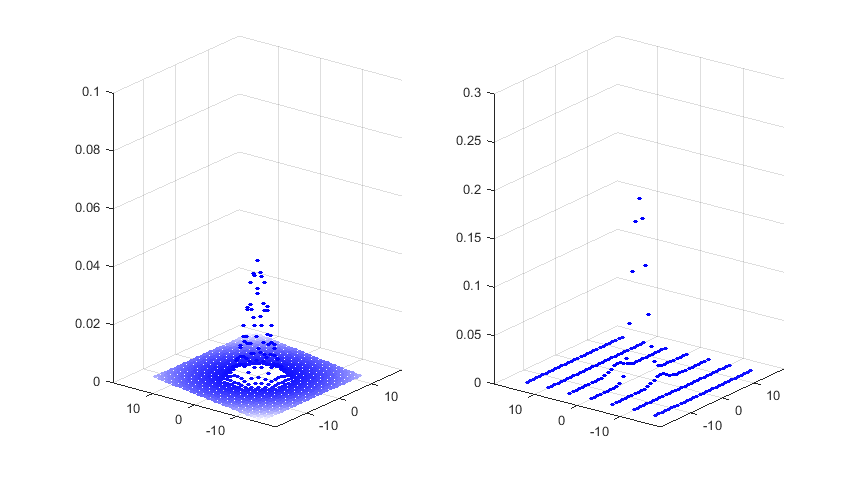
\includegraphics[scale = .45]{./figures/fig1.png}
        \caption{Gaussians with the same width over a lattice and its dual. Here the width is \(r = 5\).}
        \label{fig:Gaussian over Lattice}
    \end{figure}

\subsection{Hard Problems}
    \begin{figure}[h]
        \label{Figure: Problem Tree}
        \[\xymatrix{
            \text{GapSVP}_{\zeta, \gamma} \ar[dr]^{\text{Peikert}}\ar[d]_{\zeta\geq 2^{n/2}}&&\text{BDDP}\ar[dl]\\
            \text{GapSVP}_\gamma\ar[r]^{Q}\ar[u] &  \text{LWE}\ar[r]\ar[ur]^{???} & \text{SIS}\ar@<1ex>[l]^{\text{Q}}\\
                                &  \text{SIVP}\gamma\ar[u]^{\text{Q}}& \\
                                &  \text{SVP}_\gamma\ar[u]\ar[r]^{???} & \text{SG-PIP}\ar[l]
        }\]
        \caption{Problem Tree. The arrows indicate directions of reduction. E.g. solving SVP boils down to solving SIS. Quantum reductions are indicated with a Q. [Do not put arrows without arguing or referencing]}
    \end{figure}
    On Figure \ref{Figure: Problem Tree} we present many relations between lattice problems. In this thesis we mainly concern ourselves with the bottom part, mainly SVP\(_\gamma\). However, any attack further up in the tree would result in an attack on SVP. Therefore, the security of LWE and SIS is paramount to the security of any lattice based cryptosystem. \par
    
    Lets have a word about Ajtai. In his seminal paper\cite{Ajtai} he defined many of the hard problems that are used in lattice-based cryptography. More importantly, he showed that for many of these problems, there is a reduction from average-case to worst-case. This means that many problems related to lattices is as hard in the average case as they are in the worst case. This is an important aspect of cryptography, because if a problems only sometimes is hard, then the system is not secure. Having a reduction means that every instance of the given problem is as hard as an instance created to be as difficult to break as possible.\par
    
    A quantity which we are often interested in is the shortest vector in a given lattice. We define \(\lambda_1(\Lambda)\) (abbreviated \(\lambda_1\) when the context is clear) to be the this shortest vector. This definition can be extended to include more than one vector.
    \begin{definition}[Successive Minima]
        For a lattice \(\Lambda\), we define the \emph{\(i\)-th successive minima}
        \begin{align*}
            \lambda_i = \emph{min}\{r\suchthat\Lambda\emph{ contains } i \emph{ linearly independent vectors each of length }\leq r\}
        \end{align*}
    \end{definition}
    It is easy to see that \(0 < \lambda_1 \leq \lambda_2 \leq\dots\leq\lambda_n\). How hard these problems are depends in a large extent to which basis describes the lattice. Consider for instance a lattice \(\Lambda\) with an orthogonal basis. It is not hard \change{is it not hard?} to see that the shortest vector in such a lattice would be one of the basis vectors. We therefore have an attack in time \(O(n)\) to solve SVP. By changing the basis for a lattice to be orthogonal, or as orthogonal as possible, we might give ourselves an easier time solving SVP. However, there is no known polynomial algorithm that solves neither SIVP or SVP. By relaxing these problems to not find \emph{the} shortest vectors but only approximations, we give ourselves some room to maneuver.
    
    \begin{definition}[SVP\(_\gamma\)]
        Given a basis \(\mathcal{B}\) for a lattice \(\Lambda\), output the shortest vector \(\lambda_1\) up to a scaling factor \(\gamma\), I.e., output a non-zero vector with length \emph{at most} \(\gamma\lambda_1\).
    \end{definition}
    By choosing \(\gamma\) as large as we need to, this problem becomes trivial. Naturally, we want \(\gamma\) to be as small as possible. Current algorithms tend to have \(\gamma=\mathcal{O}(2^n)\)\needtodo{is this a proven upper limit?}, which looks like a bad approximation for something that should be short. In the way we extended the SVP to SIVP by requiring more short, linearly independent vectors, we extend the SVP\(_\gamma\) similarly:
    \begin{definition}[SIVP\(_\gamma\)]
        Given a basis \(\mathcal{B}\) of a lattice \(\lambda\), the problem SIVP\(_\gamma\) is to find \(n\) linearly independent vectors \emph{all } of length at most \(\gamma\lambda_n\)
    \end{definition}
    For this relaxed SVP-version we do have a polynomial time attack for sufficiently large approximation factor. We can use the revered LLL algorithm to recover a \(\gamma\)-approximate shortest vector in time \(O(n^6(\log B)^3\) where \(n\) is the lattice dimension, \(B\) is a bound for the euclidian length of the basis vectors and \(\gamma = O(2^n)\) \cite{Galteland}\improvement{find original source}.\par
    
    Decrypting \improvement{only talk theory?} ciphertexts in lattice based cryptography often means to find the closest vector to the given ciphertext. We therefore define the problem that describes this, again with the familiar scaling factor.
    \begin{definition}[CVP\(_\gamma\)]
    Given a basis \(\mathcal{B}\) of a lattice \(\Lambda\) and a vector \(y\in\RR\), the problem is the find a non-zero vector \(x\) such that \(||y-x||_2\leq\gamma \emph{dist}(\Lambda , y)\).
    \end{definition}
    It is intuitive that CVP and SVP should be related. We could try to use CVP to find the closest vector to 0 in the lattice, which would be the shortest vector as \(x - 0 = x\). This does not quite work as 0 is also a lattice point, and 0 will always be closest to 0 so this algorithms might output 0. We can do the reduction SVP\(\leq\)CVP as shown in Figure \ref{Fig: SVP to CVP Reduction}. 
    
    \begin{figure}
    \label{Fig: SVP to CVP Reduction}
    \begin{algorithm}[H]
    \DontPrintSemicolon
     SVP($\mathcal{B}$)\;
     \For{$i = 1 $ \KwTo $n$}{
      \(\mathcal{B}^i \leftarrow \left\{b_1,\dots ,2b_i,\dots , b_n\right\}\)\;
      \(x_i\leftarrow \) CVP(\(\mathcal{B}^i, b_i)\)\;
     }
      \Return min\(\left\{x_i - b_i\right\}\)
     
     \caption{SVP to CVP reduction.}
    \end{algorithm}
    \end{figure}
    For each iteration, the algorithms makes a new basis where element \(i\) is scaled by a factor \(2\). Then, we query a CVP oracle with this new basis and the un-scaled basis element. Without scaling, CVP would trivially return \(b_i\) in each case.\needtodo{Finish this proof}. This reduction can easily\improvement{easily?} be extended to the corresponding \(\gamma\)-approximated problems.\par
    \begin{definition}[Bounded Distance Decoding Problem]
    Let \(\mathcal{B}\) be a basis for the lattice \(\Lambda\). Given a point \(t\in\emph{span}(\mathcal{B})\) with the guarantee that \(\emph{min}_{v\in\Lambda}||v-t||\leq r\) for some known \(r\leq\lambda_1/2\), output the unique \(v\in\Lambda\) closest to \(t\).
    \end{definition}
    The BDDP problem is closely related to CVP, the only difference is that we are guaranteed that the target point is sufficiently close to a lattaice point.\needtodo{Check that this is the correct definition!}.
    
    \begin{definition}[Shortst Integer Solution (SIS)]
    Given \(\vec{a}_i\in\ZZ_q^n\), find small and non-trivial \(z_i \in\ZZ \) such that
    \begin{equation}
        \label{Eq: SIS}
        z_1\vec{a}_1 + z_2\vec{a}_2 + \dots + z_n\vec{a}_n = 0\;\;\in\ZZ_q^n
    \end{equation}
    In other words, \(\vec{z}A = 0\text{ mod } q\).
    \end{definition}
    Looking long and hard at the set 
    \begin{align*}
        \Lambda_q(A)^{\perp} := \left\{\vec{x}\in\ZZ\;|\; \vec{x}A = 0\quad\text{ mod }q\right\}
    \end{align*}
    which is the set of all solution of Equation \eqref{Eq: SIS}. It is not hard to see that this set is a lattice, and therefore solving SIS is equivalent  to finding a vector with small coefficients in the lattice \(\Lambda(A)^{\perp}\). It is important to note that this does \emph{not} mean that we find a short vector in the lattice, as a short vector can have very large coordinates. Ajtai\cite{Ajtai} showed that many lattice problems \change{Which ones?} are at least as hard as SIS (See Figure \ref{Figure: Problem Tree}. \par
    Another problem which is seemingly not related to lattices is called \emph{learning with errors}. The setup is a set of linear equations with some error.
    \begin{equation}
    \label{Equation: LWE}
        \begin{split}
            b_1 = & \;\langle \vec{s}, \vec{a}_1\rangle + e_1\\
            b_2 = & \;\langle \vec{s}, \vec{a}_2\rangle + e_2\\
            \vdots & \\
            b_k = & \;\langle \vec{s}, \vec{a}_k\rangle + e_k
        \end{split}
    \end{equation}
    where \(\vec{a}_i\leftarrow\ZZ_q^n\), the \(e_i\)-s are sampled from some distribution \(\chi\) and \(\vec{s}\in\ZZ_q^n\). The 'learning' part of the problem is to recover \(s\). Notice that without the error terms \(e_i\), this can be solved by Gaussian elimination if we have enough equations because \(\vec{A}\) will be invertible given enough equation\improvement{cite}. It is therefore natural to let \(k > n\) to have this problem make any sense. For clean notation we define a LWE-sample
    \begin{definition}
        Pick \(\vec{s}\leftarrow\ZZ_q^n\) and \(e\leftarrow\chi\). An \emph{LWE-sample} is a sample of the form \((a, b)\) where \(\vec{a}\leftarrow\ZZ_q^n\) and \( b = \langle \vec{s}, \vec{a}\rangle + e\). We say that an LWE-sample is a sample from the distribution \(A_{\vec{s}, \chi}\).
    \end{definition}
    Related to LWE are two problems; recovering\footnote[2]{Which acts like the secret key in cryptosystem based on LWE} \(\vec{s}\) and deciding whether the \(b_i\)-s are distributed according to the above selection \improvement{clearer language here} or if they are distributed uniformly.
    \begin{definition}[Search LWE]
        Given access to many LWE-samples, recover \(\vec{s}\).
    \end{definition}
    
    \begin{definition}[Decision LWE]
       Given access to many LWE-samples and \(A = (\vec{a}_1, \vec{a}_2,\dots ,\vec{a}_k)\), distinguish \((\vec{A}, \vec{b} = \vec{s}\vec{A} + \vec{e})\) from \((\vec{A}, \vec{u})\) where \(\vec{u}\) is distributed uniformly.
    \end{definition}
    
    A fact about decision-LWE and search-LWE is that they are equivalent. 
    \begin{proposition}
    search-LWE = decision-LWE
    \end{proposition}
    \begin{proof}
        \underline{search-LWE\(\leq\)decision-LWE}: This is trivial because if we can recover \(s\), then we can calculate \(\vec{e} = \vec{b} - A\vec{s}\) and check if \(\vec{e}\) is uniformly distributed. This is assuming that \(\vec{e}\) is \emph{not} uniformly distributed from the start, making decision-LWE impossible.\par
        \noindent\underline{decision-LWE\(\leq\)search-LWE}: Let \(\vec{s} = (s_1,\dots ,s_{k})\). We are going to find one coordinate of \(\vec{s}\) at a time. Pick a random \(r\leftarrow\ZZ_q\). We observe that 
        \[
            \begin{split}
                b_i' & =  \langle \vec{s}, \vec{a}_i  + (r, 0,\dots , 0)\rangle + e \\
                & = \langle \vec{s}, \vec{a}_i\rangle + s_1r + e
            \end{split}
        \]
        Now, since \(r\) was chosen uniformly at random, \(b_i'\) will also be uniformly distributed, unless \(s_1 = 0\). Therefore, we query the decision-LWE oracle on \(\big(\vec{b}^{'}, (\vec{s} + (r,0,\dots ,0))A + e\big)\). If decision-LWE decides that it is \emph{not} uniformly distributed we conclude that \(s_0 = 0\). Otherwise, we shift \improvement{Ague for shifting} \(\vec{s}\) by \(\vec{t} = (1,0, \dots, 0)\) and do that same thing with \(\vec{s} + \vec{t}\). Doing this \(q\) times will result in deciding what \(s_0\) is. Doing this for all \(s_i\) recovers \(\vec{s}\).
    \end{proof}\improvement{Can make this proof more detailed.}
    This means that we can regard both problems as one, namely LWE. We also have average case hardness of LWE.
    \begin{proposition}
        LWE is as hard in the average case as it is in the worst case.
    \end{proposition}
    \begin{proof}
        Let \(\mathcal{A}_{\vec{s}}\) denote a LWE-sample. Assume there is some set \(S\subseteq\ZZ_q^n\) such that \(|S|/|\ZZ_q^n| = 1/\text{poly}(n)\), i.e. \(S\) is not too small, and that LWE-samples where \(\vec{s}'\leftarrow S\), decision-LWE is easy. That is, we have a distinguisher \(A\) which can distinguish samples from \(\mathcal{A}_{\vec{s}'}\) from uniform ones. It is easy to see that the sample \(\{\vec{a}_i, \vec{b}_i + \langle \vec{a}_i, \vec{t}\rangle /q\}\) are samples from \(\mathcal{A}_{\vec{s}+\vec{t}}\). Therefore, given \emph{any} \(s\leftarrow\ZZ_q^n\), pick a uniformly random \(\vec{t}\leftarrow\ZZ_q^n\), and query \(A\) on 
        \begin{align*}
            \{\vec{a}_i, \vec{b}_i + \langle \vec{a}_i, \vec{t}\rangle/q\}.
        \end{align*}
        Since \(S\) is sufficiently large, we will, with high probability, eventually \(\vec{s} + \vec{t}\in S\) and we can solve the problem by querying \(A\). This means that if there exists a sufficiently large set \(S\) where decision-LWE is easy, then decision-LWE is easy \emph{for all} of \(\ZZ_q^n\). We conclude that no such set can exist \improvement{why can it not?}. Since decision-LWE \(=\) search-LWE we get that LWE is average case hard\change{Be more precise}.
    \end{proof}
    To illustrate the relationship between LWE and lattices, consider
    \begin{align*}
        \Lambda_q(A) = \left\{\vec{z}\suchthat\vec{z} = \vec{s}A\text{ mod } q \text{ for some }\vec{s}\in\ZZ_q^m\right\}.
    \end{align*}
    Given a point \(\vec{s}\vec{A}\) in the lattice \(\vec{y} = \vec{s}A + \vec{e}\) we can use CVP to recover \(\vec{s}A\) and solve \(\vec{b} = \vec{s}A\). If we also can guarantee that \(\vec{e}\) is 'short', the problem becomes BDDP.\par
    
    We now give an example of an attack on LWE. Given a LWE-sample \((\vec{a}, b = \langle \vec{s}, \vec{a}\rangle + e)\) and a divisor \(q'|q\), we can reduce the sample modulo \(q'\) to obtain
    \begin{align*}
        (\vec{a}' = \vec{a}\text{ mod } q', b' = \langle \vec{s}', \vec{a}' + e)
    \end{align*}
    where \(s' = s \text{ mod } q'\). Notice that the errors are still from the same distribution \(\chi\)\improvement{argue for this}. If we let \(q' = 1\) then \(\langle \vec{s}', \vec{a}'\rangle = 0\) so \(b = e\modulo\ZZ\). We not have two potential attacks. Firstly, if we can conclude that samples from \(\chi\) are not uniform modulo \(\ZZ\), then we have a distinguishing attack. We simply need to check whether \(b\in\RR/\ZZ\) are non-uniform.\par
    
    Secondly, we have a potential search attack. Assume that the errors from \(\chi\) usually does not wrap around modulo \(\ZZ\), that is the probability that an error is outside the interval \([-1/2, 1/2)\) is small. Symbolically,
    \begin{align*}
        \text{Pr}\left[e\not\in\left[-\frac{1}{2}, \frac{1}{2}\right)\right] \leq \varepsilon
    \end{align*}
    for a small \(\varepsilon\). We now have an attack: Let \(\Hat{e}\) be an error that does not wrap around. By definition of \(\hat{e}\), \(b - \hat{e} = \langle \vec{s}, \vec{a}\rangle\) so if we can collect enough such errors we can recover error-less LWE samples and solve LWE trivially by, for instance, Gaussian elimination. Since the probability that an error does \emph{not} wrap around is small, we can find enough such errors in short time.\par
    
    These two attack also work for other divisors of \(q\), but for simplicity we only describe it for \(q' = 1\).\improvement{why do we know these divisors?}. From these two attack we get two requirements for the error distribution \(\chi\): It must be statistically indistinguishable from uniform modulo \(\ZZ\), and the sufficiently many errors must wrap around modulo \(\ZZ\).\par
    
    If we not let \(\chi = D_r\) be a Gaussian of width \(r\) exceeding the smoothing parameter \(r \geq \eta_\varepsilon(\ZZ)\). We can for instance let \(r > \sqrt{n} \geq \eta_{2^{-n}}(\ZZ)\) as described in the worst-case hardness theorems from LWE\needtodo{find these sources, ez}. These errors wrap around modulo \(\ZZ\) with high probability \improvement{cite} and moreover \(b\modulo\ZZ\) are statistically close to uniform by the choice of the width of \(D_r\). 
    
\subsection{Ring-LWE}
    Before we discuss Ring-LWE we want to have a low-level discussion of a vector space. We define \(K_\RR := K\otimes\RR\). By fixing a \(\QQ\)-basis for \(K\), \(\{u_1, \dots , u_n\}\) such that we can write any \(\alpha\in K\) as \(\alpha = q_1u_1 + \dots + q_n u_n\). Now any element \(e\in K_\RR\) is of the form
    \begin{align*}
        e = (q_1, q_2, \dots , q_n)\otimes x = (q_1x,q_2x,\dots ,q_nx)
    \end{align*}
    for \(q_i\in\QQ\) and \(x\in\RR\). Since \(q_i x\in\RR\), we get that \(K_\RR\) is a vector space over \(\RR\) and hence isomorphic to \(\RR^n\). The vector space \(K_\RR\) is where the errors are drawn in the ring variant of LWE.\par
    
    For applications, \(\vec{s}\) is the secret key in cryptosystems based on LWE. Now, to have any chance of recovering \(\vec{s}\) we need to have more than \(n\) equations, so \(m = O(n)\) at least. The key size is therefore \(O(n^2)\) which is pretty big. As introduced in \cite{First R-LWE}, it is desirable to, instead of sampling from \(\ZZ_q^n\), sample from a certain ring. 
    \begin{definition}[Ring-LWE (R-LWE)]
        Let \(\OO_q = \OO/\langle q\rangle\). Pick a secret \(s\in \OO_q^\vee\). Let \(\chi\) be a distribution over \(K_{\RR}\). Sample \(a \leftarrow \OO_q\) uniformly and \(b\leftarrow (a\cdot b) + e \emph{ mod } qR^\vee\). A R-LWE sample is \((a, b)\). As before, the \emph{search} version is the recover \(s\) and the \emph{decision} version is to distinguish a R-LWE sample \((a, b)\) from one where \(b\) is sampled uniformly.
    \end{definition}
    Notice that the secret key is an element from the dual lattice \(\OO^\vee\). This will be discussed later. However, a definition where the samples are all taken from the non-dual \(\OO\) is equivalent to this definition, up to the error distribution \(\chi\)\cite{How Not To RLWE}. There is some 'tweaking' needed for this equivalence\needtodo{cite}. From Proposition \ref{Prop: Cancel Ideal} we have that\needtodo{convince yourself that this is the consequence of this prop!} there exists an bijection
    \begin{align*}
        \theta_t : \OO_q^\vee\rightarrow \OO_q,
    \end{align*}
    which we can extend to a map
    \begin{align*}
        \kappa_t:K_\RR/q\OO^\vee\rightarrow K_\RR/q\OO
    \end{align*}
    naturally. We use \(\kappa_t\) to transform a R-LWE sample \((a_i, b_i = s\cdot a_i + e_i)\) by
    \begin{align*}
        b_i' = \kappa_t(b_i) = t\cdot b_i = s'\cdot a_i + e_i'
    \end{align*}
    and keeping \(a_i\) fixed. \improvement{is it fixed or is the map on \(a_i\) fixed?} Notice that \(\kappa_t(s) = \theta_t(s)\), and since \(\theta_t\) is a bijection, we get that \(s'\) is distributed uniformly (since \(s\) was). This is therefore a valid R-LWE sample with error distribution \(t\cdot\chi\). Because \(\theta_t\) is a bijection, finding \(s'\) immidiately yields \(s\), so solving search for the transformed sample (with errors from \(t\cdot\chi\)) is equivalent to solving search for the original samples. Additionally, because \(\kappa_t\) sends uniform samples to uniform samples \needtodo{check} we get that the decision versions are equivalent as well.\par
    
    The cruical thing to note now is that we have a \emph{new} error distribution \(t\cdot\chi\). So if \(\chi\) itself satisfies the hardness properties of R-LWE, \(t\cdot\chi\) might not. The important part for hardness is the length of the errors. Consider therefore \(e\leftarrow\chi\). Under \(\kappa_t\) this becomes \(t\cdot e\) and has norm
    \begin{equation*}
        \begin{split}
            ||te|| = ||\sigma(te)|| & = ||(\sigma_1(te),\dots ,\sigma_n(te)||\\
                                    & = ||(\sigma_1(t)\sigma_1(e), \dots ,\sigma_n(t)\sigma_n(e)|| 
        \end{split}
    \end{equation*}
    In the trivial case where \(t\in\ZZ\) we get that \(t\cdot\chi\) is just a scaled version of \(\chi\), meaning a spherical distribution remains spherical. In general, however, \(t\in\OO^\vee\). Now if \(\chi\) is spherical, \(t\cdot\chi\) need not be since each \(i\)-th coordinate is scaled by \(\sigma_i(t)\). If the reductions rely on the \emph{largest} width of the Gaussians, we might try to scale each coordinate by the largest \(\sigma_i(t)\) such that we get a spherical distribution. However, this means that we need to change other parameters of the system to guarantee security. This is why keys from \(\OO_q^\vee\) makes for the tightest bounds and is the 'right' choice of ring.\par
    
    It is not obvious that R-LWE has the same hardness-properties as LWE, in particular a reduction from worst-case to average-case. However, R-LWE is connected to LWE in the following sense. If we let \(\mathcal{B}\) be a basis for \(R\), then for any \(a\in R_q\), we get that multiplication by \(a\) is represented by a matrix relative to the basis, say \(\vec{A}_a\). So given any \(s\in R_q\), we can represent it with respect to \(\mathcal{B}\) as \(\vec{s}\in \ZZ_q^n\). Now, given a R-LWE sample \((a, b = s\cdot a + e)\) we get \(n\) LWE samples
    \begin{align*}
        (\vec{A}_a, \vec{b} = \vec{s}\vec{A}_a + \vec{e}).
    \end{align*}
    It is not obvious now what the distribution of the columns of \(\vec{A}_a\) are uniformly distributed or that \(\vec{e}\) are. One attack on R-LWE makes sure that for any sample, we transform it into an \emph{error-less} LWE-sample. If we can generate enough of these, we can recover \(\vec{s}\) by linear algebra. \change{Move and make cohesive}\par
    
    Now, depending on how well we can represent the elements of \(R\), this version of LWE reduces the key-size by a factor of \(n\)\cite{First R-LWE}. However, we have introduced different structure on the sets we sample from. It is therefore not apparent that we have equally strong security on R-LWE as we do for 'regular' LWE. However, \cite{How Not To RLWE} shows that we can get as strong security on R-LWE as we did for LWE. In addition, under some assumptions we can get that search- and decision-R-LWE are equivalent.\par
    
    This relation between LWE and R-LWE is what is used in the security proof of certain instantiations of R-LWE. \par
    
    However, in \cite{First R-LWE} it was shown that we do indeed have similar properties. There is a \emph{quantum} reduction from worst-case SVP\(_\gamma\) on ideal lattices to the search variant of R-LWE. In addition, the R-LWE distributions are pseudorandom, meaning that the decision version of R-LWE is hard. These two properties are captured in the following theorem:
    \begin{theorem}[\cite{First R-LWE}]
        Suppose that it is hard for polynomial-time quantum algorithms to approximate the search version of the approximate SVP in the worst case on ideal lattices in \(\OO\) to within a fixed poly(n) factor. Then any poly(n) number of samples drawn from the distribution are pseudoreandom to any polynomial-time (possibly quantum) attacker.
    \end{theorem}
    
    We now describe two attacks, one one search and one on decision, of R-LWE from \cite{How Not To RLWE}. Both attacks are very similar to the attacks on 'regular' LWE. Let \(\frakq\) be an ideal divisor of \(\OO\). Given R-LWE samples
    \begin{align*}
        (a_i, b_i = s\cdot a_i + e_i)
    \end{align*}
    we transform them into samples modulo \(\frakq\) by setting \(a_i' = a_i \text{ mod } \frakq\) and \(b_i' = b_i \text{ mod } \frakq\). Now, \(b_i' = s'\cdot a_i' + e_i\) for \(s' = s\text{ mod } \frakq\). We have that reduction modulo \(\frakq\) maps uniform samples to uniform samples\needtodo{Argue for this?}. Now if \(\chi\text{ mod }\frakq\) is detectably non-uniform, we immediately have a distinguishing attack. For each candidate \(\hat{s}\in \OO/\frakq\) for \(s'\) check whether \(b_i' - \hat{s}\cdot a_i'\) are non-uniform. If such an \(\hat{s}\) exists, conclude that the distribution on the original \(b_i\) is \emph{not} uniform.\par
    
    If \(\chi\) has one or more coordinates that does not 'wrap around' modulo \(\ZZ\), then we can attack search by reducing the R-LWE samples to error-less LWE samples. If we can do this enough times we can solve LWE by, e.g., Gaussian elimination. \par
    
    We described an attack on LWE above, by reducing the samples modulo a divisor of \(q\). We can extend this attack to R-LWE by using a similar approach. Given an ideal divisor \(\frakq\) of \(q\OO\) we reduce the R-LWE samples to
    \begin{align*}
        (a_i'\modulo \frakq , b_i' = b_i\modulo \frakq).
    \end{align*}
    We have that \(a_i'\in\OO/\frakq\) and \(b_i' \in \RR^n/\frakq\OO ^\vee\). For each of the \(N(\frakq)\) candidates of the reduced secret \(s'\in\OO^\vee/\frakq\OO^\vee\), we check whether \(b_i' - a_i\cdot s'\in\RR^n/\frakq\OO^\vee\) are non-uniform. Like we assumed for simplicity that the divisor \(q'|q\) be \( q' = 1\), we now let \(\frakq = \OO\), such that we get maximum reduction:
    \begin{equation*}
        \begin{split}
            a' = & 0\modulo\OO^\vee\\
            b' = & e\modulo\OO^\vee
        \end{split}
    \end{equation*}
    Now, checking whether \(e\in K_{\RR}\) is non-uniform we have a distinguishing attack. If the error \(e\) does not 'wrap around', then we can reduce the samples to error-less LWE-samples and trivially recover the secret \(s\). 'Wrapping around' in this context means that the coefficients of the error vector \(\vec{e}\) corresponding to \(e\) via an appropriate basis does not wrap around. However, if we can guarantee that neither of these conditions are satisfied for a distribution \(\chi\), then none of these attacks work. Indeed, choosing a Gaussian with fitting width will be sufficient for both these conditions.\par
    
    We describe the reduction from the BDDP to R-LWE under certain conditions on the parameters. However, we show this reduction for a slightly different BDDP.
    \begin{definition}
        The \(q\)-BDDP\(_{\calI, d}\) is: given an instance \(y\) of BDD\(_{\calI, d}\) that has solution \(x\), find \(x\modulo q\calI\)
    \end{definition}
    Regev showed in \cite{Reg05} that there is a polynomial time reduction from BDDP\(_{\calI, d}\) to \(q\)-BDDP\(_{\calI, d}\). This means that we want to prove the second reduction in Figure \ref{fig:BDD to R-LWE Reduction}.
    \begin{figure}
        \[
        \xymatrix{\text{BDD}\ar[r] & q\text{-BDDP}\ar[r] & \text{R-LWE}}
        \]
        \caption{BDD to R-LWE reduction.}
        \label{fig:BDD to R-LWE Reduction}
    \end{figure}
    So, given a \(q\)-BDDP\(_{\calI^\vee, d}\) instance \(y = x + e\) with \(x\in\calI^\vee\) we want to make use of an R-LWE oracle \(\mathcal{L}\) and a DGS oracle \(\mathcal{D}_{\calI, r}\) to recover \(x\). Start by computing \(t\) such that \(t\cdot\calI\inverse\) is coprime to \(\langle q \rangle\). Now we use the R-LWE oracle \(\mathcal{L}\) as follows: \(\mathcal{L}\) will request samples untill it is confident that it has a solution. For each of these requets, sample \(z\leftarrow\mathcal{D}_{\calI, r}\) and compute the pair \((a, b)\) by
    \begin{equation*}
        \begin{split}
            a = &\theta_t\inverse (z\modulo q\calI) \\
            b = &(z\cdot y)/q + e'\modulo\OO^\vee.
        \end{split}
    \end{equation*}
    \needtodo{Talk about CRT, \(\theta(a)\) etc.}When we have helped \(\mathcal{L}\) enough times, it will output \(s\in\OO^\vee\). Finally compute \(\theta_t\inverse(s) \in \calI_q^\vee\). We now argue for correctness. To do this, prove that the \(a\) above is statistically close to uniform and the \(b\) is statistically close to a spherically bounded Gaussian.
    
\subsection{Why using \(\OO^\vee\) is Right}
    \begin{itemize}
        \item Emerges naturally from the BDD-to-LWE reduction from \cite{First R-LWE}.
        
        \item Good for cryptography: Allows for most errors while still decrypting correctly. Hardness theorems from \cite{First R-LWE} assume \emph{dual version} of R-LWE. Instantiating with 'correct' parameters but \emph{non-dual version} means that the tweak factor ruins the sperical error distribution.
        
        \item Natural for standard SIS-LWE 
    \end{itemize}
    


\subsection{Instantiating R-LWE}
     We can describe how to instantiate R-LWE in such a way that the attacks in \cite{How Not To RLWE} perform no better than known attacks (e.g. \cite{LWE Attack 1, LWE Attack 2}) against 'normal' LWE instantiated to have worst case hardness. This means that the width of the Gaussian is \(r>2\sqrt{n}\). We do this by relating parameters for R-LWE to LWE in such a way that we have sufficient parameters corresponding to the hardness-condition for worst-case hardness \emph{of LWE}. \par
     
     The following theorem is the only quantum step in some reductions regarding LWE and R-LWE:
     \begin{theorem}
        Let \(\alpha > 0\) and \(q\leq 2\) be an integer. There exists an efficient quantum algorithm that, given a fractional ideal \(\fraka\subseteq K\) and a number \(r\leq\sqrt{2}\cdot\eta_{\varepsilon}(\fraka)\) for some negligible \(\varepsilon = \varepsilon(n)\) such that \(r' := r\cdot\omega(\sqrt{\log n})/(\alpha q)\), an oracle to R-LWE\(_{q, \Psi_{\leq\alpha}}\), and a list of samples from the discrete Gaussian distribution \(D_{\fraka, r}\) outputs an independent sample from \(D_{\fraka, r'}\).
     \end{theorem}
     This theorem describes an iterative step for sampling from \(D_{r'}\) given enough samples from \(D_{r}\) where \(r' < r\). Additionally, we have a reduction from BDD to R-LWE for certain parameters. 